\documentclass{beamer}

\mode<presentation>
{
  \usetheme{Wolfenbuettel}
  \setbeamercovered{transparent}
}


\usepackage[english]{babel}

\usepackage[latin1]{inputenc}

%\usepackage{times}
\usepackage{ae}
\usepackage[T1]{fontenc}
\usepackage{euler}

\usepackage{jkmath}

\usepackage{array}

\setbeamertemplate{title page}
{ 
  \begin{centering}
    \begin{beamercolorbox}[sep=8pt,center,colsep=-4bp,rounded=true,shadow=true]{title}
      \usebeamerfont{title}\inserttitle\par
      \vskip0.25em           
      {\usebeamerfont{subtitle}\usebeamercolor[fg]{subtitle}\insertsubtitle\par}
    \end{beamercolorbox}
    \begin{beamercolorbox}[sep=8pt,center,colsep=-4bp,rounded=true,shadow=true]{author}
      \usebeamerfont{author}\insertauthor
    \end{beamercolorbox}
    \begin{beamercolorbox}[sep=8pt,center,colsep=-4bp,rounded=true,shadow=true]{date}
      \usebeamerfont{date}\insertdate
    \end{beamercolorbox}\vskip0.5em
  \end{centering}  
}


\title{Nonequispaced Fast Spherical Fourier Transform and Applications}

\author
{Jens Keiner}

%\institute[Universit�t zu L�beck]
%{Institut f�r Mathematik}

%\date[Oberseminar]{Oberseminar Mathematik, 29.06.2005}

%\subject{Numerical Analysis}

% If you have a file called "university-logo-filename.xxx", where xxx
% is a graphic format that can be processed by latex or pdflatex,
% resp., then you can add a logo as follows:

%\pgfdeclareimage[height=0.5cm]{university-logo}{gridsphere}
%\logo{\pgfuseimage{university-logo}}


% Delete this, if you do not want the table of contents to pop up at
% the beginning of each subsection:
%\AtBeginSubsection[]
%{
%  \begin{frame}<beamer>
%    \frametitle{Outline}
%    \tableofcontents[currentsection,currentsubsection]
%  \end{frame}
%}


% If you wish to uncover everything in a step-wise fashion, uncomment
% the following command: 

%\beamerdefaultoverlayspecification{<+->}


\begin{document}

\begin{frame}
  \titlepage
  \begin{figure}[h]
    \centering
    \includegraphics[width=0.3\textwidth]{sh_r_9_5}
  \end{figure}
\end{frame}

\begin{frame}
  \frametitle{Outline}
  \tableofcontents[pausesections]
  % You might wish to add the option [pausesections]
\end{frame}


% Structuring a talk is a difficult task and the following structure
% may not be suitable. Here are some rules that apply for this
% solution: 

% - Exactly two or three sections (other than the summary).
% - At *most* three subsections per section.
% - Talk about 30s to 2min per frame. So there should be between about
%   15 and 30 frames, all told.

% - A conference audience is likely to know very little of what you
%   are going to talk about. So *simplify*!
% - In a 20min talk, getting the main ideas across is hard
%   enough. Leave out details, even if it means being less precise than
%   you think necessary.
% - If you omit details that are vital to the proof/implementation,
%   just say so once. Everybody will be happy with that.

\section{Fourier Analysis on \twosphere}

\begin{frame}
  \frametitle{Spherical Coordinates}

  \begin{itemize}
  \item
    $\V{x} \in \R^3 \setminus \set{\V{0}}$
  \item
    $\V{x} = \paren{x_1,x_2,x_3}^{\transp} = \paren{r \sin \vtheta \cos \vphi, r \sin \vtheta \sin \vphi, r \cos \vtheta}^{\transp}$,\\ $r \in \Rp$, $\vtheta \in \interv{[}{0}{\pi}{]}$, $\vphi \in \interv{[}{0}{2\pi}{)}$
  \end{itemize}

  \begin{figure}[h]
    \centering
    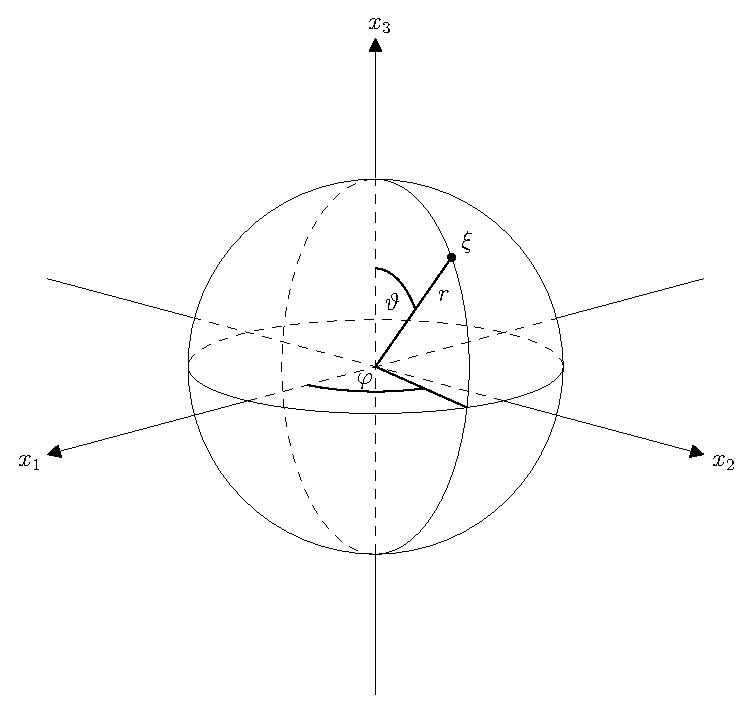
\includegraphics[width=0.5\textwidth]{sphere}
  \end{figure}

\end{frame}

\begin{frame}
  \frametitle{Comparison $\mathbb{S}^1$ and $\twosphere$}

  \newcolumntype{C}{>{$}c<{$}} 
  \newcolumntype{L}{>{$}l<{$}} 
  \newcolumntype{R}{>{$}r<{$}} 
  \setlength{\extrarowheight}{5pt}

  {\tiny
  \begin{tabular}{|l|C|C|}
    \firsthline
               & \mathbb{S}^1 & \twosphere \\[5pt] \hline
    Definition & \mathbb{S}^1 := \mathbb{T}^1 := \pset{\V{x} \in \R^2}{|}{\norm{\V{x}}_{2} = 1} &
    \twosphere := \pset{\V{x} \in \R^{3}}{|}{\norm{\V{x}}_2 = 1} \\[5pt] \hline
    Laplace's equation & \frac{\partial^2}{\partial x_1^2} + \frac{\partial^2}{\partial x_2^2} = 0 &
    \frac{\partial^2}{\partial x_1^2} + \frac{\partial^2}{\partial x_2^2} + \frac{\partial^2}{\partial x_3^2} = 0 \\[5pt]
                       & \lasthline
  \end{tabular}
  }

  You can create overlays\dots
  \begin{itemize}
  \item using the \texttt{pause} command:
    \begin{itemize}
    \item
      First item.
      \pause
    \item    
      Second item.
    \end{itemize}
  \item
    using overlay specifications:
    \begin{itemize}
    \item<3->
      First item.
    \item<4->
      Second item.
    \end{itemize}
  \item
    using the general \texttt{uncover} command:
    \begin{itemize}
      \uncover<5->{\item
        First item.}
      \uncover<6->{\item
        Second item.}
    \end{itemize}
  \end{itemize}
\end{frame}


\subsection{Previous Work}

\begin{frame}
  \frametitle{Make Titles Informative.}
\end{frame}

\begin{frame}
  \frametitle{Make Titles Informative.}
\end{frame}



\section{Nonequispaced Fast Spherical Fourier Transform (NFSFT)}

\subsection{Main Results}

\begin{frame}
  \frametitle{Make Titles Informative.}
\end{frame}

\begin{frame}
  \frametitle{Make Titles Informative.}
\end{frame}

\begin{frame}
  \frametitle{Make Titles Informative.}
\end{frame}


\subsection{Basic Ideas for Proofs/Implementation}

\begin{frame}
  \frametitle{Make Titles Informative.}
\end{frame}

\begin{frame}
  \frametitle{Make Titles Informative.}
\end{frame}

\begin{frame}
  \frametitle{Make Titles Informative.}
\end{frame}

\section{Applications}

\section*{Summary}

\begin{frame}
  \frametitle<presentation>{Summary}

  % Keep the summary *very short*.
  \begin{itemize}
  \item
    The \alert{first main message} of your talk in one or two lines.
  \item
    The \alert{second main message} of your talk in one or two lines.
  \item
    Perhaps a \alert{third message}, but not more than that.
  \end{itemize}
  
  % The following outlook is optional.
  \vskip0pt plus.5fill
  \begin{itemize}
  \item
    Outlook
    \begin{itemize}
    \item
      Something you haven't solved.
    \item
      Something else you haven't solved.
    \end{itemize}
  \end{itemize}
\end{frame}



% All of the following is optional and typically not needed. 
\appendix
\section<presentation>*{\appendixname}
\subsection<presentation>*{For Further Reading}

\begin{frame}[allowframebreaks]
  \frametitle<presentation>{For Further Reading}
    
  \begin{thebibliography}{10}
    
  \beamertemplatebookbibitems
  % Start with overview books.

  \bibitem{Author1990}
    A.~Author.
    \newblock {\em Handbook of Everything}.
    \newblock Some Press, 1990.
 
    
  \beamertemplatearticlebibitems
  % Followed by interesting articles. Keep the list short. 

  \bibitem{Someone2000}
    S.~Someone.
    \newblock On this and that.
    \newblock {\em Journal of This and That}, 2(1):50--100,
    2000.
  \end{thebibliography}
\end{frame}

\end{document}


